\documentclass[10.5pt]{article} % For LaTeX2e
\usepackage{times}
\usepackage{lscape} 
\usepackage{hyperref}
\usepackage{longtable}
\usepackage{amsmath}
\usepackage{graphicx} % Required for inserting images
\usepackage{url}
\usepackage{rotating}
\usepackage{booktabs}
\usepackage{tabularx}
\usepackage{geometry}
\usepackage{float}
\usepackage{placeins}
\geometry{a4paper, margin=1in}
\usepackage[backend=bibtex]{biblatex}
\addbibresource{references.bib} % Add the bibliography file
\usepackage[a4paper, margin=0.7in , top=0.5in]{geometry} 

\title{
  \textbf{Robust Bayesian Inference for the Censored Mixture of Experts Model Using Heavy-Tailed Distributions}\\[0.5em]
  \textit{Elham Mirfarah,Mehrdad Naderi, Tsung-I Lin, Wan-Lun Wang} \\[0.5em]
  \large MTH422 Course Project
}
\author{
  Ahana Bose (231080009) \\
  Sneha Karmakar (231080087) \\
  Sohini Bhadra (231080089) \\
  Rishikesh Dargad (220891)
}
\date{Course Instructor : Prof. Arnab Hazra\\[0.5em]20 April 2025}



    

\newcommand{\fix}{\marginpar{FIX}}
\newcommand{\new}{\marginpar{NEW}}


\begin{document}

\maketitle
\thispagestyle{empty}

\tableofcontents
\newpage



\section{Introduction}

Censored data, where responses are only partially observed, frequently occurs in fields like biomedicine, clinical trials, and econometrics. Traditional regression models often assume normally distributed errors, making them sensitive to outliers and latent heterogeneity, which can lead to poor estimation and classification performance.\\

\noindent
The Mixture of Experts (MoE) model addresses heterogeneity by dividing data into subgroups, each with its own regression structure. However, standard MoE models still rely on normality assumptions and are not well-equipped to handle censoring or heavy-tailed distributions.\\

\noindent
To overcome these limitations, this study proposes a \textbf{Bayesian Mixture of Experts (MoE)} model with \textbf{Scale Mixture of Normal (SMN)} errors, allowing for more robust handling of outliers and extreme values. The model, called \textbf{MoE-SMN-CR}, supports left, right, and interval censoring. It uses \textbf{Ultimate Pólya-Gamma (UPG)} augmentation to efficiently estimate gating parameters and perform posterior inference.

\noindent
Simulation studies and real data analysis demonstrate that the proposed Bayesian approach improves estimation accuracy, classification performance, and robustness compared to traditional likelihood-based methods.

\section{Model specification and Bayesian inference}

\subsection{Notation and background material}

Throughout this paper, we use the following notations:

\begin{itemize}
    \item $\phi(\cdot; \mu, \sigma^2)$ and $\Phi(\cdot; \mu, \sigma^2)$ denote the probability density function (pdf) and cumulative distribution function (cdf) of the normal distribution $\mathcal{N}(\mu, \sigma^2)$, respectively.
    \item $\text{Gamma}(\alpha, \eta)$ is the gamma distribution with mean $\alpha/\eta$.
    \item $\text{IG}(\alpha, \eta)$ represents the inverse-gamma distribution with mean $\eta/(\alpha - 1)$.
    \item $\text{TN}(\mu, \sigma^2; (a, b))$ and $\text{TG}(\alpha, \eta; (a, b))$ denote the truncated normal and truncated gamma distributions on the interval $(a, b)$, respectively.
    \item $\mathcal{U}(a, b)$ is the uniform distribution over the interval $(a, b)$.
    \item $\text{BE}(\alpha, \eta)$ is the beta distribution with mean $\alpha / (\alpha + \eta)$.
\end{itemize}

\noindent
The class of Scale Mixture of Normal (SMN) distributions is defined by scaling the variance of a normal variable using a positive mixing random variable. A random variable $Y \sim \text{SMN}(\mu, \sigma^2, \nu)$ admits the following stochastic representation:
\[
\bm{Y} \overset{d}{=} \bm{\mu} + \bm{U}^{-1/2} \bm{Z}
\]
where $Z \sim \mathcal{N}(0, \sigma^2)$ and $U \sim H(\cdot; \nu)$ are independent, and $\overset{d}{=}$ denotes equality in distribution. The parameter $\nu$ controls the tail behavior of the SMN distribution.

\noindent
Alternatively, the hierarchical form is given by:
\[
Y \mid (U = u) \sim \mathcal{N}(\mu, u^{-1}\sigma^2), \quad U \sim H(u; \nu).
\]

\noindent
Thus, the pdf of the SMN distribution can be expressed as:
\[
\bm{f}_{\text{\textbf{SMN}}}(\bm{y}; \bm{\mu}, \bm{\sigma}^2, \bm{\nu}) 
= \int_{\bm{0}}^{\bm{\infty}} \bm{\phi}(\bm{y}; \bm{\mu}, \bm{u}^{-1} \bm{\sigma}^2) \, d\bm{H}(\bm{u}; \bm{\nu}), 
\quad \bm{y} \in \bm{\mathbb{R}}.
\]

\noindent
The SMN class provides a flexible tool for robust statistical modeling. It includes several well-known heavy-tailed distributions as special cases, such as the Student's $t$, Slash, Contaminated Normal, Laplace, Variance-Gamma, and Tail-Inflated Normal distributions. 
\subsection{Model formulation}

Suppose the random errors in the Mixture of Experts (MoE) model follow the Scale Mixture of Normal (SMN) distribution. Then, the probability density function (pdf) of the MoE-SMN model can be written as:
\[
f(y_i; \bm{\Theta}) = \sum_{j=1}^{g} \pi_j(\bm{r}_i; \bm{\tau}) 
f_{\text{SMN}}\left(y_i; \bm{x}_i^\top \bm{\beta}_j, \sigma_j^2, \nu_j\right), 
\quad i = 1, \dots, n,
\]

\newpage

\noindent
where:
\begin{itemize}
    \item $\Theta = (\boldsymbol{\theta}_1, \dots, \boldsymbol{\theta}_g, \boldsymbol{\tau})$ is the collection of all model parameters,
    \item $\boldsymbol{\theta}_j = (\boldsymbol{\beta}_j, \sigma_j^2, \nu_j)$ are the parameters of the $j$-th expert,
    \item $\pi_j(\mathbf{r}_i; \boldsymbol{\tau})$ is the gating function given by the multinomial logistic link:
    \[
    \pi_j(\mathbf{r}_i; \boldsymbol{\tau}) = \frac{\exp(\boldsymbol{\tau}_j^\top \mathbf{r}_i)}{1 + \sum_{\ell=1}^{g-1} \exp(\boldsymbol{\tau}_\ell^\top \mathbf{r}_i)}, \quad j = 1, \dots, g-1,
    \]
    and $\pi_g(\mathbf{r}_i; \boldsymbol{\tau}) = 1 - \sum_{j=1}^{g-1} \pi_j(\mathbf{r}_i; \boldsymbol{\tau})$.
\end{itemize}

\noindent
To account for censoring, assume that for each observation we observe $(c_i, \rho_i)$, where:
\begin{itemize}
    \item $c_i$ is the observed value: either the actual response if uncensored ($y_i = c_i$), or the censoring threshold if $y_i \leq c_i$,
    \item $\rho_i$ is the censoring indicator: $\rho_i = 0$ if uncensored, and $\rho_i = 1$ if censored.
\end{itemize}

\noindent
Then, the likelihood function under left-censoring is given by:
\[
L(\Theta \mid \mathbf{y}_{\text{obs}}, \boldsymbol{\rho}) = \prod_{i=1}^{n} \sum_{j=1}^{g} \pi_j(\mathbf{r}_i; \boldsymbol{\tau}) \left[ \sigma_j^{-1} f_{\text{SMN}}(e_{ij}; \nu_j) \right]^{1 - \rho_i} \left[ F_{\text{SMN}}(e_{ij}^c; \nu_j) \right]^{\rho_i},
\]
where:
\[
e_{ij} = \frac{y_i - \mathbf{x}_i^\top \boldsymbol{\beta}_j}{\sigma_j}, \quad 
e_{ij}^c = \frac{c_i - \mathbf{x}_i^\top \boldsymbol{\beta}_j}{\sigma_j}.
\]

\noindent
To facilitate Bayesian computation, a hierarchical representation is used:
\[
\begin{aligned}
Y_i \mid (Z_{ij} = 1, U_i = u_i) &\sim \mathcal{N}(\mathbf{x}_i^\top \boldsymbol{\beta}_j, u_i^{-1} \sigma_j^2), \\
U_i \mid (Z_{ij} = 1) &\sim H(u; \nu_j), \\
\mathbf{Z}_i \mid \mathbf{r}_i &\sim \text{Multinomial}(1; \pi_1(\mathbf{r}_i; \boldsymbol{\tau}), \dots, \pi_g(\mathbf{r}_i; \boldsymbol{\tau})).
\end{aligned}
\]

\noindent
This hierarchical form allows efficient sampling in a Bayesian framework using data augmentation strategies.

\subsection{Priors and Hyper-parameter Specifications}

In Bayesian analysis, priors incorporate prior knowledge from previous observations, offering important insights. For clarity and computational efficiency, we employ conjugate and improper priors in our MoE-SMN-CR model. Conjugate priors are beneficial as their posteriors remain within the same distribution family, streamlining calculations while preserving interpretability.

\noindent
Assuming prior independence among all parameters $\{\boldsymbol{\theta}_1, \ldots, \boldsymbol{\theta}_g, \boldsymbol{\tau} \}$, the joint prior distribution factorizes as:
\[
\pi(\Theta) = \prod_{j=1}^{g} \pi(\boldsymbol{\beta}_j)\, \pi(\sigma_j^2)\, \pi(\nu_j) \times \prod_{j=1}^{g-1} \pi(\boldsymbol{\tau}_j).
\]

\noindent
The specific prior distributions are as follows:
\begin{itemize}
   \item \textbf{Regression Coefficients:} For each expert $j = 1, \ldots, g$, the regression coefficients $\boldsymbol{\beta}_j$ follow a multivariate normal prior:
\[
\boldsymbol{\beta}_j \sim \mathcal{N}_p(\mathbf{0}, \kappa_\beta^2 \mathbf{I}_p),
\]
where $\kappa_\beta^2$ is a large constant (e.g., 100 or 1000) and $\mathbf{I}_p$ is the $p \times p$ identity matrix.


    \item \textbf{Gate Function Parameters:} To enable efficient inference for the multinomial logistic regression governing the gating network, we employ the Pólya-Gamma (PG) data augmentation technique proposed by Polson et al.\ (2013). Specifically, we assign:
    \[
    \boldsymbol{\tau}_j \sim \mathcal{N}_q(\mathbf{0}, 2000\, \mathbf{I}_q), \quad j = 1, \ldots, g - 1,
    \]
    where $\boldsymbol{\tau}_j$ are the gating coefficients and $\mathbf{I}_q$ denotes the $q \times q$ identity matrix. These priors are weakly informative and facilitate posterior inference via the PG augmentation framework.

    \item \textbf{Pólya-Gamma Data Augmentation:} A random variable $\omega \sim \text{PG}(\xi_1, \xi_2)$ admits the following stochastic representation:
    \[
    \omega \overset{d}{=} \frac{1}{2\pi^2} \sum_{k=1}^\infty \frac{g_k}{(k - 0.5)^2 + \xi_2^2 / (4\pi^2)},
    \]
    where $g_k \sim \text{Gamma}(\xi_1, 1)$ are i.i.d.\ gamma variables. For a PG-distributed $\omega$, the binomial likelihood involving a log-odds term $\psi$ satisfies the identity:
    \[
    \frac{e^{a \psi}}{(1 + e^\psi)^{\xi_1}} = 2^{-\xi_1} e^{\kappa \psi} \int_0^\infty e^{-\omega \psi^2 / 2} f(\omega; \xi_1)\, d\omega, \quad \text{with } \kappa = a - \xi_1 / 2.
    \]
    This representation transforms the binomial likelihood into a conditionally Gaussian form, enabling efficient Gibbs updates.

    \item \textbf{Ultimate Pólya-Gamma Sampling:} To further enhance sampling efficiency and reduce posterior autocorrelation, we utilize the Ultimate Pólya-Gamma (UPG) sampler . This extension optimizes latent variable sampling and improves mixing in hierarchical mixture models such as MoE-SMN-CR.
\end{itemize}


\subsection{Full Conditional Posteriors}

Due to the complex likelihood structure, the marginal posterior distributions of the parameters are analytically intractable. MCMC methods, such as Gibbs sampling and the Metropolis-Hastings (MH) algorithm, can be employed to generate posterior samples from the full conditional distributions. The full conditional distribution of each parameter, including latent variables, given the value of all remaining ones, is required. Below, we outline how the MCMC algorithm, coupled with a data-augmentation scheme, is used to obtain the full conditional distribution of each parameter in the model:

\begin{itemize}
    \item \textbf{Step 1:} Sample the mixing random variable $U_i$ conditioning on all parameters and latent variables in the model.
    \begin{itemize}
        \item The full conditional distribution of $U_i$ given $(y_i, Z_i, \dots)$ is determined through the distribution of the mixing random variable $U$.
    \end{itemize}
    
    \item \textbf{Step 2:} Treat $m$ censored values as missing data.
    \begin{itemize}
        \item For a left-censored observation $c_k$, the conditional distribution of $Y_k$ is:
        \[
        Y_k \mid (y_k < c_k, Z_k = 1, u_k, \beta_j, \sigma_j^2) \sim \text{TN}(x_k \beta_j, u_k^{-1} \sigma_j^2; (-\infty, c_k]),
        \]
        where $k = 1, \dots, m$.
        \item For right-censored observations, the truncation interval switches to $[c_k, +\infty)$.
    \end{itemize}
    
    \item \textbf{Step 3:} Simulate samples of $\beta_j$ for $j = 1, \dots, g$ from the posterior distribution:
\[
\beta_j \mid (y_{\text{obs}}, Z, \mathbf{u}, \Theta_{(-j)}, \sigma_j^2) \sim \mathcal{N}_p \left( \tilde{\Sigma}_{\beta_j} \left[ \sigma_j^{-2} \left( \sum_{i=1}^n z_{ij} u_i y_i x_i^\top \right) + \Sigma_{\beta_j}^{-1} b_{\beta_j} \right], \, \tilde{\Sigma}_{\beta_j} \right),
\]
where $\Theta_{(-j)}$ denotes all parameters excluding $\beta_j$, and
\[
\tilde{\Sigma}_{\beta_j} = \left( \sigma_j^{-2} \sum_{i=1}^n z_{ij} u_i x_i x_i^\top + \Sigma_{\beta_j}^{-1} \right)^{-1}.
\]

    \item \textbf{Step 4:} Draw samples of $\sigma_j^2$ for $j = 1, \dots, g$ from the posterior distribution:
    \[
    \sigma_j^2 \mid (y_{\text{obs}}, Z, u, \Theta_{(-j)}, \beta_j) \sim \text{IG} \left( a_{\sigma_j} + \sum_{i=1}^n z_{ij}, \quad b_{\sigma_j} + \sum_{i=1}^n z_{ij} u_i (y_i - x_i^\top \beta_j)^2 \right),
    \]
    where $\text{IG}(\cdot, \cdot)$ denotes the inverse-gamma distribution, and $\Theta_{(-j)}$ represents all parameters excluding the $j$-th component.

    \item \textbf{Step 5:} Sample $\nu_j$ based on the assumed mixing distribution $H(u; \nu)$ and its prior specification.
    \begin{itemize}
        \item The procedure for sampling $\nu_j$ depends on the specific form of the mixing distribution. Implementation details for different cases are given in Section 2.5 of the main text.
    \end{itemize}

    \item \textbf{Step 6:} Draw samples of the latent cluster indicator $Z_i$ from its posterior distribution:
    \[
    Z_i \mid (y_i, r_i, \cdots) \sim \mathcal{M}(1; p^{\text{Bayes}}_{i1}, \dots, p^{\text{Bayes}}_{ig}),
    \]
    where $\mathcal{M}$ denotes the multinomial distribution with one trial, and
    \[
    p^{\text{Bayes}}_{ij} = \frac{\pi_j(r_i; \tau_j) \, f_{\text{SMN}}(y_i; x_i^\top \beta_j, \sigma_j^2, \nu_j)}{\sum_{l=1}^g \pi_l(r_i; \tau_l) \, f_{\text{SMN}}(y_i; x_i^\top \beta_l, \sigma_l^2, \nu_l)},
    \]
    where $f_{\text{SMN}}$ is the density function of the skewed multivariate normal distribution.

    \begin{itemize}
        \item For censored observations, Step 2 is used to impute values for $y_i$.
        \item If $Z_{ij} = 1$, the $i$-th observation is assigned to the $j$-th component.
    \end{itemize}

    \item\textbf{EM-based Posterior Membership Probabilities:} \\
    When using the EM algorithm, the posterior membership probability of the $i$-th sample belonging to group $j$ is given by:
    \[
    p^{(EM)}_{ij} = \frac{\pi_j(r_k; \tau_j) f_{\text{SMN}}(\epsilon^{c}_{i,j})}{\sum_{l=1}^g \pi_l(r_k; \tau_l) f_{\text{SMN}}(\epsilon^{c}_{i,l})},
    \]
    for $k = 1, \dots, m_d$, where $\epsilon^{c}_{i,j}$ is the latent residual corresponding to the censored observation, as defined in Equation (4) of the original text. This expression involves evaluating the cdf of the SMN distribution at the censoring threshold.

    \item \textbf{Step 7:} Sample $\tau$ using the UPG (Uncollapsed Polya-Gamma) sampler for multinomial data.
    \begin{itemize}
        \item The $g$-th group is used as the baseline category.
        \item Sampling follows ``Algorithm 2'' in Zens et al.\ (2023), employing a three-level hierarchical update scheme, described in Appendix E of the supplementary material.
    \end{itemize}

\end{itemize}
These full conditionals allow efficient implementation of a Gibbs sampler (with Metropolis-Hastings steps as needed) for posterior inference under the proposed Bayesian MoE-SMN-CR model.

\subsection{Sampling Strategy for the Indexing Parameter}

In the MoE-SMN-CR model, each expert (component) is associated with a specific error distribution from the Scale Mixture of Normals (SMN) family. These distributions are parameterized by an \textbf{indexing parameter} $\nu_j$, which determines the heaviness of the tail — i.e., how robust each expert is to extreme observations. The parameter $\nu_j$ is critical in adjusting the behavior of the distribution to handle outliers effectively.\\

\noindent
Since $\nu_j$ affects the mixing distribution in the SMN formulation, its posterior distribution often lacks a closed form, requiring specialized sampling methods. Depending on the distributional form (Slash, Contaminated Normal, Student's $t$, Variance-Gamma, or Tail-Inflated Normal), different strategies are adopted for posterior inference. Some distributions (like Slash or CN) allow conjugate updates, while others require Metropolis-Hastings (MH) algorithms. In what follows, we describe the approach for each distribution in detail.

\subsubsection{Slash (SL) Distribution}
The Slash distribution is a simple heavy-tailed distribution that arises from dividing a standard normal variable by a uniform variable. When a conjugate prior $\nu_j \sim \text{Gamma}(a_{\nu_j}, b_{\nu_j})$ is assigned, the posterior conditional distribution of $\nu_j$ is also a Gamma, allowing for direct Gibbs sampling.

\[
\nu_j \mid \cdot \sim \text{Gamma} \left( a_{\nu_j} + \sum_i z_{ij},\ b_{\nu_j} - \sum_i z_{ij} \log u_i \right)
\]

\noindent
This closed-form update is computationally convenient and ensures rapid convergence during MCMC sampling.

\subsubsection{Contaminated Normal (CN) Distribution} 
The CN model introduces robustness by mixing two normal distributions — one for regular observations and one with inflated variance to accommodate outliers. Here, $\nu_j$ represents the mixing proportion and is modeled using a Beta prior, while an auxiliary variable $\gamma_j$ determines the contamination threshold and is drawn from a Uniform(0,1) prior.

\[
\nu_j \sim \text{Beta}(a_{\nu_j}, b_{\nu_j}), \quad \gamma_j \sim \text{Uniform}(0,1)
\]

\noindent
The full conditionals are:

\[
\nu_j \mid \cdot \sim \text{Beta} \left( a_{\nu_j} + \sum_i \frac{z_{ij}(1 - u_i)}{1 - \gamma_j},\ b_{\nu_j} + \sum_i \frac{z_{ij}(u_i - \gamma_j)}{1 - \gamma_j} \right)
\]

\[
\gamma_j \mid \cdot \sim \text{TG} \left( \frac{1}{2} \sum_i b_{ij} z_{ij} + 1,\ \frac{1}{2} \sum_i b_{ij} z_{ij} e_{ij}^2;\ (0,1) \right)
\]

\noindent
where $b_{ij} = 1$ if $u_i \leq \gamma_j$ and $0$ otherwise. This hierarchical setup allows different experts to handle varying contamination levels, improving clustering robustness.

\subsubsection{Student’s $t$ Distribution} 
The Student’s $t$ distribution is widely used for its ability to model heavy tails with a single parameter $\nu_j$. However, no closed-form exists for the full conditional of $\nu_j$. Thus, two distinct strategies are proposed: the \textbf{Hierarchical} (Hier) method and the \textbf{Non-Hierarchical} (non-Hier) method.

\vspace{1em}

\noindent
\textbf{Hierarchical Method:} \\
\noindent
This method relies solely on the latent scale variables $u_i$, making it computationally efficient, but less informative as it does not use the observed response $y_i$. The log-posterior is expressed as:

\[
\pi(\nu_j \mid \cdot) \propto \left(\frac{\nu_j}{2}\right)^{\sum_i z_{ij}} \Gamma\left(\frac{\nu_j}{2}\right)^{-\sum_i z_{ij}} 
\prod_i u_i^{z_{ij}(\nu_j/2 - 1)} \exp\left(-\frac{\nu_j}{2} \sum_i z_{ij} u_i\right) \pi(\nu_j)
\]

\noindent
We construct a second-order Taylor expansion:

\[
q(\nu_j) = \frac{\nu_j}{2} \sum_i z_{ij} \log \left(\frac{\nu_j}{2} \right) - \sum_i z_{ij} \log \Gamma\left( \frac{\nu_j}{2} \right) 
- \frac{\nu_j}{2} \sum_i z_{ij} \left(u_i - \log u_i \right) + \log \pi(\nu_j)
\]

\noindent
From $q(\nu_j)$, a truncated normal proposal is defined:

\[
\nu_j^{\text{new}} \sim \text{TN}(\mu_\nu, \sigma_\nu^2; (2, 40)), \quad 
\mu_\nu = \nu_j - \frac{q'(\nu_j)}{q''(\nu_j)}, \quad \sigma_\nu^2 = -\frac{1}{q''(\nu_j)}
\]

\noindent
The MH acceptance probability becomes:

\[
\alpha = \min \left( 1,\ \frac{\exp(q(\nu_j^{\text{new}})) \cdot p(\nu_j)}{\exp(q(\nu_j)) \cdot p(\nu_j^{\text{new}})} \right)
\]
\noindent
\textbf{Non-Hierarchical Method:} \\
This method improves robustness by incorporating full data likelihood (including $y_i$, censoring, and gating functions). The posterior becomes:

\[
q(\nu_j) = \log(\pi(\nu_j)) + \sum_i \log \left[ \pi_j(r_i; \tau) 
f_T(y_i; x_i^\top \beta_j, \sigma_j^2, \nu_j)^{1 - \rho_i} 
F_T(c_i; x_i^\top \beta_j, \sigma_j^2, \nu_j)^{\rho_i} \right]
\]
\noindent
Several priors for $\nu_j$ can be used:
\begin{itemize}
\item \textbf{Jeffreys prior:} 
\[
\pi(\nu_j) \propto \left( \frac{\nu_j}{\nu_j + 3} \right)^{1/2}
\left[ \psi'\left(\frac{\nu_j}{2}\right) - \psi'\left(\frac{\nu_j + 1}{2}\right) \right]
- \frac{2(\nu_j + 3)}{\nu_j(\nu_j + 1)^2}
\]
\item \textbf{Truncated Gamma:} $\nu_j \sim \text{TG}(a_{\nu_j}, b_{\nu_j};\ (2, 40])$
\item \textbf{Pareto:} $\pi(\nu_j) \propto \frac{2}{\nu_j^2},\ \nu_j \geq 2$
\item \textbf{Juárez and Steel Prior:}
\[
\pi(\nu_j) \propto \frac{\nu_j - 1}{\left(\nu_j - 1 + \frac{4}{1+\sqrt{2}} \right)^3}, \quad \nu_j \geq 1
\]
\end{itemize}

\noindent
This method is more informative and leads to better inference, particularly in heterogeneous datasets.

\subsubsection{Variance-Gamma (VG) Distribution} 
This distribution supports similar hierarchical and non-hierarchical methods. \begin{itemize}
    \item \textbf{Hierarchical Approach:}  
    For the Variance-Gamma (VG) distribution, the indexing parameter $\nu_j$ can be sampled using hierarchical (Hier) and non-hierarchical (non-Hier) methods, similar to the approach used for the Student's $t$ distribution.

    In the Hierarchical approach, the full conditional distribution is proportional to:
    \[
    \pi(\nu_j \mid Z, u, \text{others}) \propto 
    \left\{ \left( \frac{\nu_j}{2} \right)^{\frac{\nu_j}{2}} \frac{1}{\Gamma\left( \frac{\nu_j}{2} \right)} \right\}^{\sum_{i=1}^n z_{ij}} 
    \cdot \nu_j^{a_{\nu_j} - 1} \cdot \exp\left( -\frac{\nu_j}{2b_{\nu_j}} \right) \cdot \mathbb{I}_{(0, 40)}(\nu_j),
    \]
    where $\mathbb{I}_{(0, 40)}(\cdot)$ is the indicator function ensuring $\nu_j \in (0, 40)$.

    \item \textbf{Non-Hierarchical Approach:}  
    For the non-Hierarchical case, the conditional posterior distribution becomes:
    \[
    \pi(\nu_j \mid y_{\text{obs}}, \rho, \text{others}) \propto \pi(\nu_j) \prod_{i=1}^n 
    \left[ f_{\text{VG}}(y_i; x_i \beta_j, \sigma_j^2, \nu_j)^{z_{ij}(1 - \rho_i)} 
    \cdot \left( \frac{\pi_j(r_i; \tau)}{F_{\text{VG}}(c_i; x_i \beta_j, \sigma_j^2, \nu_j)} \right)^{z_{ij} \rho_i} \right],
    \]
    where:
    \begin{itemize}
        \item $f_{\text{VG}}(\cdot)$ is the density function of the VG distribution,
        \item $F_{\text{VG}}(\cdot)$ is its cumulative distribution function (cdf),
        \item $\rho_i = 1$ if $y_i$ is censored and $0$ otherwise,
        \item $c_i$ is the censoring threshold for $y_i$.
    \end{itemize}
\end{itemize}

\subsubsection{Tail-Inflated Normal (TIN) Distribution} 
This recently proposed distribution inflates the tails of a normal distribution using a random threshold. Assuming a prior $\nu_j \sim \text{Uniform}(0, 1)$, the full conditional becomes:

\[
\pi(\nu_j \mid \cdot) \propto \left( \frac{1}{\nu_j} \right)^{\sum_i z_{ij}} 
\mathbb{I}_{(1 - \min_{z_{ij}=1} u_i,\ 1)}(\nu_j)
\]
\noindent
Since this does not belong to a known family, sampling is performed using MH.

\subsubsection{Laplace and Normal Distributions}
Both of these are special cases in the SMN class where the tail behavior is fixed. As they do not involve an indexing parameter $\nu_j$, no sampling is needed for these components.

\vspace{1em}
\noindent
Conjugate updates are available in limited cases, but more commonly, MH-based methods are employed. Hierarchical modeling allows each expert to adaptively learn its robustness from the data, enhancing interpretability and performance in real-world applications where outliers and non-Gaussian noise are prevalent.

\newpage

\section{Simulations}
\subsection{Comparison of MH Strategies for Sampling Indexing Parameters in MoE-T-CR and MoE-VG-CR Models}

\subsubsection{Objective}
The primary objective of this simulation study is to compare the effect of the proposed Metropolis-Hastings (MH) strategies for sampling indexing parameters in the MoE-T-CR (Mixture of Experts with T-distribution Censored Responses) and MoE-VG-CR (Mixture of Experts with Variance-Gamma Censored Responses) models. The focus is on evaluating the variation of the estimated indexing parameters under two different scenarios:

\begin{itemize}
    \item \textbf{Equal scenario} where the parameters \( \nu_1 = \nu_2 = \nu_3 = 5 \).
    \item \textbf{Unequal scenario} where the parameters \( (\nu_1, \nu_2, \nu_3) = (3, 6, 10) \).
\end{itemize}

\subsubsection{Methodology}
To evaluate the performance of the proposed MH strategies, a total of 100 Monte Carlo (MC) samples of size 500 were generated from the three-component MoE-T-CR and MoE-VG-CR models. The following parameter values were specified for the simulation:

\[
\begin{aligned}
    &\beta_1 = (0, 4), \quad \beta_2 = (0, -3), \quad \beta_3 = (-2, 1), \quad (\sigma_1^2, \sigma_2^2, \sigma_3^2) = (0.2, 0.1, 0.2) \\
    &\tau_1 = (-2, 4), \quad \tau_2 = (-2, -4)
\end{aligned}
\]

\noindent
The covariates were generated as \( r_i = (1, x_{1i}) \), where \( x_{1i} \) was drawn from a uniform distribution \( U(-2, 2) \).

\noindent
For each synthetic dataset, a left-censoring scheme with a level of 15\% was implemented, following the generation algorithm described in Mirfarah et al. (2021).

\subsubsection{MCMC Sampling}
The MCMC sampling procedure was conducted to obtain Bayesian estimates of the indexing parameters. Convergence was typically achieved after collecting 20,000 MCMC samples, with the initial 5,000 iterations discarded as burn-in. The posterior mean of the indexing parameters was computed for each converged MCMC sample.\\
\noindent
The experiment was repeated over 100 replications to obtain reliable estimates. The Bayesian estimates were used to compute various accuracy metrics, which are discussed below.

\subsubsection{Accuracy Metrics}
The performance of the estimation method was assessed using the following metrics:

\begin{itemize}
    \item \textbf{Standard Deviation (STD):} The variability of the estimated indexing parameters.
    \item \textbf{Absolute Relative Bias (ARB):} The absolute difference between the true value of \( \nu_j \) and its Bayesian estimate, normalized by the true value. It is defined as:
\end{itemize}

\[
\text{ARB}_j = \frac{1}{100} \sum_{k=1}^{100} \left| \frac{\hat{\nu_j}^{(k)} - \nu_j}{\nu_j} \right|
\]

\noindent
Where \( \hat{\nu_j}^{(k)} \) is the Bayesian estimate (posterior mean) of \( \nu_j \) obtained at the \( k^{\text{th}} \) sample.

\begin{itemize}
    \item \textbf{Root Relative Mean Squared Error (RRMSE):} The root mean square error of the Bayesian estimate, normalized by the true value. It is defined as:
\end{itemize}

\[
\text{RRMSE}_j = \sqrt{\frac{1}{100} \sum_{k=1}^{100} \left( \frac{\hat{\nu_j}^{(k)} - \nu_j}{\nu_j} \right)^2}
\]
\begin{figure}[H]
    \centering
    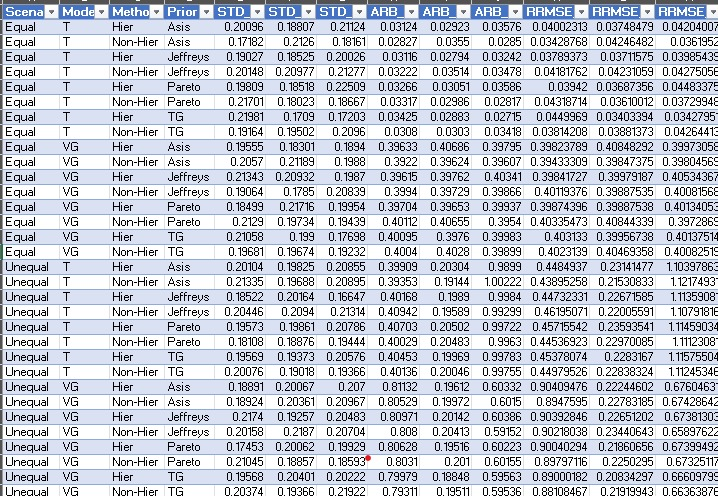
\includegraphics[width=1\textwidth]{WhatsApp Image 2025-04-20 at 17.11.48.jpeg} % Replace with your image file name and extension
    \caption{Simulation results for assessing sampling strategies for the indexing parameter in the MoE-T-CR and MoE-VG-CR models for “equal" and “unequal" scenarios}
    \label{fig:your_label} % Optional: for referencing the figure
\end{figure}

\subsection{Interpretation}

\subsubsection{Equal Variance Scenario}

\paragraph{T-Distribution Models}
\begin{itemize}
    \item The T-distribution models demonstrate superior performance across all prior specifications, with RRMSE values consistently below 0.05 for all parameters (v1, v2, v3).
    \item Hierarchical models with "TG" priors yield the lowest RRMSE for parameters v2 (0.034) and v3 (0.034), suggesting optimal performance for these parameters.
    \item Non-hierarchical models with "Asis" priors perform best for parameter v1 (RRMSE = 0.034), indicating that different model specifications may be optimal for different parameters.
    \item The standard deviations (STD) across all T-distribution models remain relatively stable (ranging from 0.17 to 0.22), indicating consistent precision regardless of prior choice.
\end{itemize}

\paragraph{VG-Distribution Models}
\begin{itemize}
    \item VG-distribution models perform substantially worse than T-distribution models, with RRMSE values approximately 10 times higher (around 0.40) across all parameters.
    \item The average absolute bias (ARB) for VG models is dramatically higher (approximately 0.39–0.40) compared to T models (approximately 0.03–0.04).
    \item This substantial performance gap suggests that VG-distribution models are inappropriate for data with equal variance characteristics.
\end{itemize}

\subsubsection{Unequal Variance Scenario}

\paragraph{T-Distribution Models}
\begin{itemize}
    \item Under unequal variance conditions, T-distribution models show parameter-specific performance patterns:
    \begin{itemize}
        \item For v1: RRMSE values increase to approximately 0.44–0.46
        \item For v2: RRMSE values increase moderately to approximately 0.22–0.24
        \item For v3: RRMSE values increase dramatically to approximately 1.10–1.12
    \end{itemize}
    \item The substantially higher RRMSE for v3 indicates that this parameter is particularly sensitive to variance heterogeneity.
    \item Prior choice becomes more influential under unequal variance, though no single prior consistently outperforms others across all parameters.
\end{itemize}

\paragraph{VG-Distribution Models}
\begin{itemize}
    \item Interestingly, VG models show improved relative performance under unequal variance compared to equal variance scenarios:
    \begin{itemize}
        \item For v1: RRMSE values are high (approximately 0.88–0.90)
        \item For v2: RRMSE values are comparable to T models (approximately 0.21–0.23)
        \item For v3: RRMSE values are lower than T models (approximately 0.66–0.68)
    \end{itemize}
    \item This suggests that while VG models remain suboptimal overall, they may offer advantages for specific parameters (particularly v3) when variances are unequal.
\end{itemize}

\subsubsection{Hierarchical vs. Non-Hierarchical Modeling}
\begin{itemize}
    \item In the equal variance scenario, hierarchical modeling provides marginal improvements for T-distribution models with certain priors, but the benefits are not consistent across all parameters and prior specifications.
    \item Under unequal variance conditions, the performance difference between hierarchical and non-hierarchical approaches becomes even less pronounced, suggesting limited practical advantage to hierarchical modeling in this context.
\end{itemize}

\subsubsection{Prior Sensitivity}
\begin{itemize}
    \item For T-distribution models with equal variance, the "Jeffreys" prior offers the most balanced performance across all parameters.
    \item For unequal variance scenarios, prior choice has a more substantial impact, though no single prior demonstrates clear superiority.
    \item The sensitivity to prior specification increases under challenging estimation conditions (unequal variance), highlighting the importance of careful prior selection in complex modeling scenarios.
\end{itemize}

\subsection{Comparison of Bayesian and EM-based Inferences}

The Bayesian approach can potentially offer improved clustering performance, especially when dealing with censored response variables. To evaluate this, we conduct a comparative analysis between our proposed Bayesian inference method and the likelihood-based Expectation-Maximization (EM) algorithm.

\noindent
In this experiment, we generate synthetic datasets of size \( n = 500 \) from a parallel 3-component Mixture of Experts model with Skewed Mixture Normal-Censored Regression (MoE-SMN-CR) structure. The true parameter values used in the simulation are as follows:

\begin{itemize}
    \item \textbf{Regression coefficients:} \\
    \( \boldsymbol{\beta}_1 = (10, 4), \quad \boldsymbol{\beta}_2 = (0, 4), \quad \boldsymbol{\beta}_3 = (-10, 4) \)
    
    \item \textbf{Gating network coefficients:} \\
    \( \boldsymbol{\tau}_1 = (-2, 4), \quad \boldsymbol{\tau}_2 = (-2, -4) \)
    
    \item \textbf{Error variances:} \\
    \( \sigma_1^2 = \sigma_2^2 = \sigma_3^2 = 1 \)
\end{itemize}

\noindent
Covariates are defined as \( \boldsymbol{x}_i = (1, x_{1i}) \) and \( \boldsymbol{r}_i = (1, r_{1i}) \), where both \( x_{1i} \) and \( r_{1i} \) are independently drawn from a uniform distribution \( U(-2, 2) \).
\noindent
To ensure a fair comparison between the two inference methods, the mixing variable \( U_i \) is simulated from the Generalized Inverse Gaussian (GIG) distribution, as introduced by Good (1953).\\

\noindent
The indexing parameters for the three components are:\\
\( \boldsymbol{\nu}_1 = (-0.5, 1, 0.2), \quad \boldsymbol{\nu}_2 = (0.5, 1, 0.2), \quad \boldsymbol{\nu}_3 = (-0.5, 1, 0.2) \)\\

\noindent
This setup yields samples from a mixture of symmetric geometric hyperbolic distributions, enabling a robust comparison of the clustering performance achieved by the Bayesian and EM-based approaches.

\begin{figure}[h!]
    \centering
    \begin{minipage}{0.48\textwidth}
        \centering
        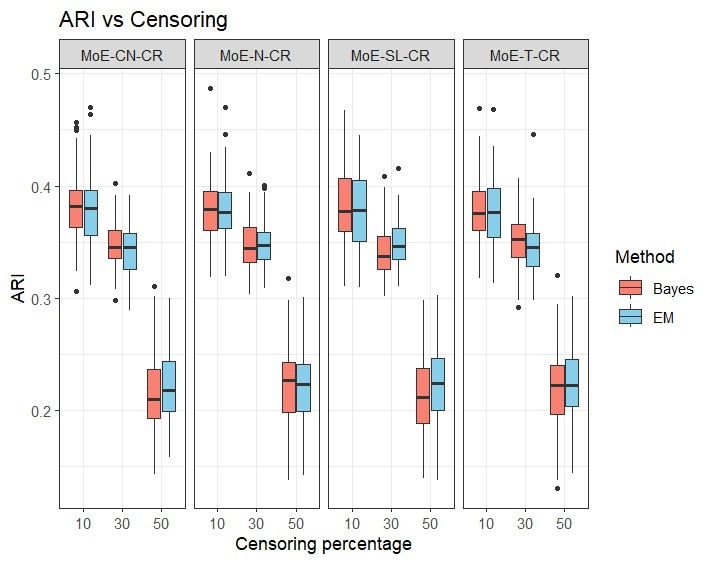
\includegraphics[width=\textwidth]{WhatsApp Image 2025-04-18 at 19.58.36.jpeg}
    \end{minipage}
    \hfill
    \begin{minipage}{0.48\textwidth}
        \centering
        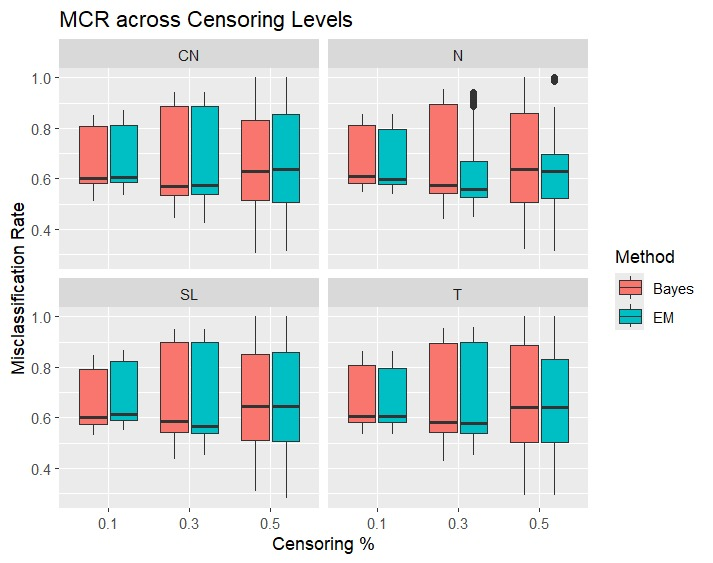
\includegraphics[width=\textwidth]{WhatsApp Image 2025-04-18 at 19.57.34 (1).jpeg}
    \end{minipage}
    \caption{Comparison of the likelihood inference via EM algorithm and Bayes method for four particular cases of the MoE-SMN-CR model in terms of the MCR and ARI scores}
\end{figure}
\subsection{Interpretation}

As censoring increases from 10\% to 50\%, clustering performance deteriorates, evidenced by a steady decline in Adjusted Rand Index (ARI) and a corresponding rise in Misclassification Rate (MCR) across all models. \textcolor{red}{Bayesian methods (red)} consistently outperform \textcolor{blue}{EM algorithms (blue)}, offering higher median ARI and lower MCR with reduced variability. Among the models, heavy-tailed error distributions—specifically \texttt{MoE-T-CR}, \texttt{MoE-SL-CR}, and \texttt{MoE-CN-CR}—demonstrate superior robustness compared to the Gaussian model \texttt{MoE-N-CR}. Notably, \texttt{MoE-CN-CR} tends to deliver the best performance in both ARI and MCR metrics. Overall, Bayesian MCMC approaches paired with heavy-tailed models provide the most accurate and stable clustering results under varying levels of censoring.


\subsection{Sensitivity Analysis of Parameter Estimation in the Presence of Outliers}

An additional simulation study was conducted to assess the robustness of the proposed Bayesian estimation procedure under data contamination. Robustness of estimation methods in the presence of outliers has been extensively studied in the literature using approaches such as case-deletion diagnostics, local influence, perturbation analysis, and contamination-based studies. Following this tradition, our objective here is to investigate the stability of parameter estimates when the response variable is subject to outliers.

\vspace{1em}

\noindent
To perform this analysis, 100 Monte Carlo samples were generated, each consisting of $n = 500$ observations drawn from a 5-component Mixture of Experts with Normal experts and Censored Regression (MoE-N-CR) model. The true parameter values for the simulation are specified as follows:

\newpage

\noindent
\textbf{Expert coefficients:}
\begin{align*}
\beta_1 &= (6, -2, 3, 2, -3),\quad 
\beta_2 = (-3, 1, 1, -2, 2),\quad 
\beta_3 = (3, -1.5, -2, -2, -1),\\
\beta_4 &= (-0.5, -2, 3, 3, -2),\quad 
\beta_5 = (-6, -2, -1, -3, 2)
\end{align*}

\vspace{1em}

\noindent
\textbf{Gating parameters:}
\begin{align*}
\tau_1 &= (1, 0.5, -1.5, 2), \\
\tau_2 &= (2, -0.2, 2, 1), \\
\tau_3 &= (-2, 3, -2, 1), \\
\tau_4 &= (-2, -3, -0.7, -2)
\end{align*}

\vspace{1em}

\noindent
\textbf{Error variances:} \quad $(\sigma_1^2, \sigma_2^2, \sigma_3^2, \sigma_4^2, \sigma_5^2) = (1, 2, 2, 1, 3)$.

\vspace{1em}

\noindent
The covariates for the experts and gating functions were generated as:
\[
x_i = (1, x_{1i}, x_{2i}, x_{3i}, x_{4i}), \quad r_i = (1, r_{1i}, r_{2i}, x_{4i}),
\]
where
\[
x_{1i} \sim U(-1,1), \quad x_{2i} \sim \text{Poisson}(2), \quad x_{3i} \sim \mathcal{N}(0,1), \quad x_{4i} \sim U(-2,2), \quad r_{1i}, r_{2i} \sim \mathcal{N}(0,1).
\]

\vspace{1em}

\noindent
To simulate the presence of outliers, a contamination process was applied by randomly selecting $\delta \in \{10, 20, 40, 60\}$ observations from each sample and replacing their corresponding responses with values generated outside the typical range of the original responses. Specifically, for a contaminated response $y_i^*$, we generated:
\[
y_i^{(\text{out})} \sim U(-20,-15)\,\mathbb{I}_{(-\infty,0)}(y_i^*) + U(15,20)\,\mathbb{I}_{[0,\infty)}(y_i^*),
\]

\vspace{1em}

ensuring the outliers lie significantly outside the data’s natural support.

\vspace{1em}
\noindent
Subsequently, seven variations of the MoE-SMN-CR model were fitted to both the uncontaminated and contaminated datasets. The resulting parameter estimates from the clean and contaminated datasets are denoted by $\hat{\theta}$ and $\hat{\theta}^{(\delta)}$, respectively.

\vspace{1em}
\noindent
To quantify the sensitivity of parameter estimation to contamination, we computed the Mean Magnitude of Absolute Error (MMAE) for the regression and gating parameters:

\vspace{1em}

\[
\text{MMAE}(\beta) = \frac{1}{25} \sum_{j=1}^{5} \sum_{l=1}^{5} \left| \hat{\beta}_{lj}^{(\delta)} - \hat{\beta}_{lj} \right|, \quad
\text{MMAE}(\tau) = \frac{1}{16} \sum_{j=1}^{4} \sum_{l=1}^{4} \left| \hat{\tau}_{lj}^{(\delta)} - \hat{\tau}_{lj} \right|.
\]

\vspace{1em}

\noindent
These metrics evaluate the deviation in parameter estimates due to contamination, thereby serving as a robustness measure for the Bayesian estimation method under consideration.

\begin{figure}[H]
    \centering
    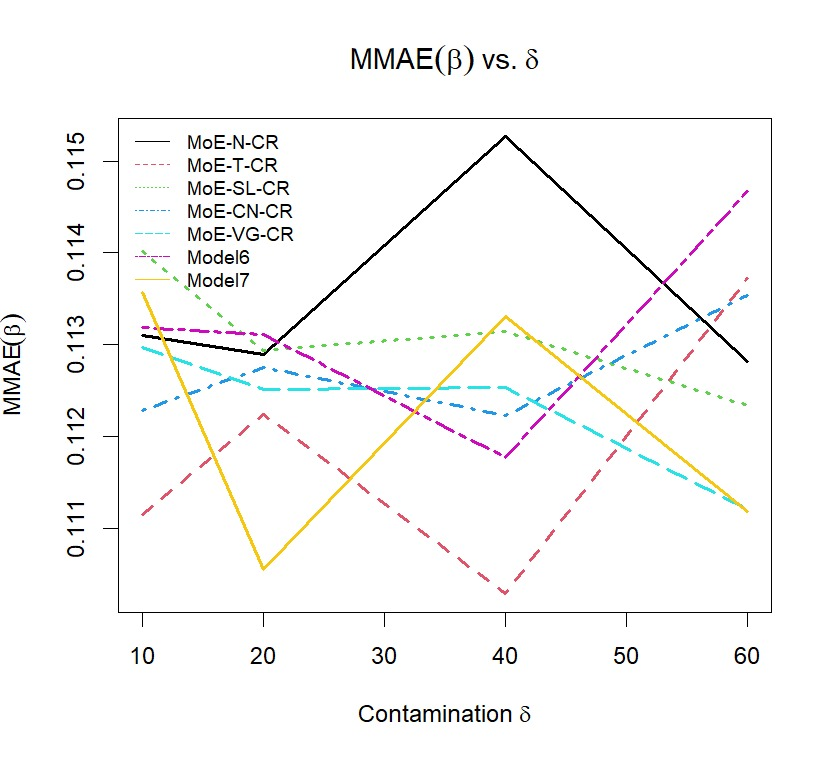
\includegraphics[width=0.75\textwidth]{WhatsApp Image 2025-04-20 at 12.48.14.jpeg}
    \caption{Average MMAE as a function of contamination level ($\delta$) for the covariate $\beta$.}
\end{figure}
\begin{figure}[H]
    \centering
    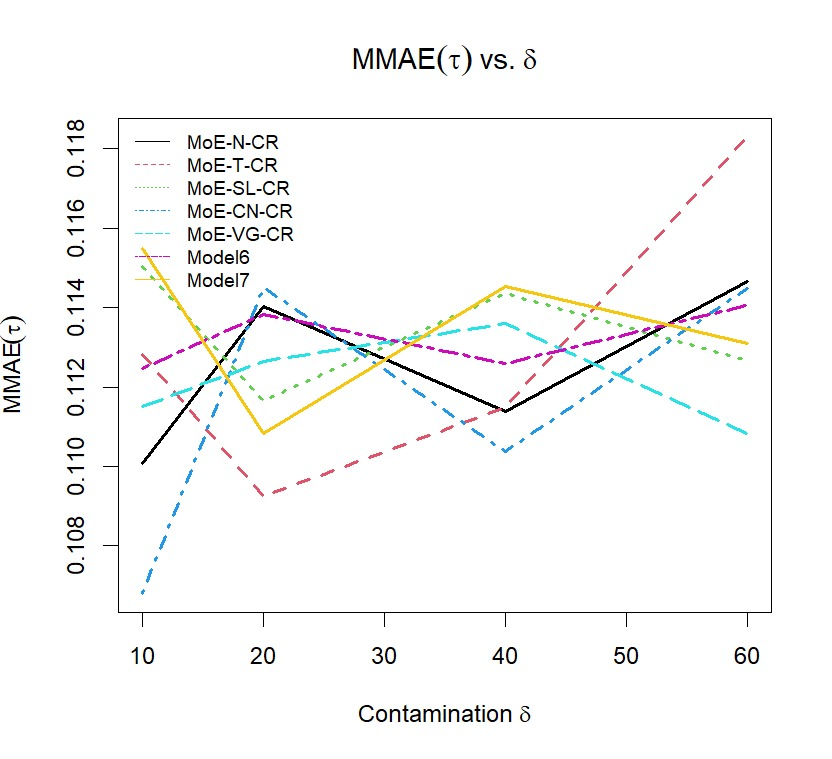
\includegraphics[width=0.75\textwidth]{mmae.jpg}
    \caption{Average MMAE as a function of contamination level ($\delta$) for the gating parameter $\tau$.}
\end{figure}

\subsubsection{Interpretation}
\begin{itemize}
  \item \textbf{MMAE($\beta$) vs.\ $\delta$:}
    \begin{itemize}
      \item The Gaussian model (MoE‑N‑CR) exhibits a marked increase in error as contamination grows, indicating low robustness.
      \item Heavy‑tailed/skewed models (MoE‑T‑CR, MoE‑SL‑CR, MoE‑CN‑CR, MoE‑VG‑CR) show nearly flat MMAE($\beta$) curves; MoE‑SL‑CR and MoE‑CN‑CR are the most stable.
      \item Reference models (Model6, Model7) lie between Gaussian and heavy‑tailed variants in sensitivity.
    \end{itemize}

  \item \textbf{MMAE($\tau$) vs.\ $\delta$:}
    \begin{itemize}
      \item MoE‑N‑CR error increases monotonically with outlier level.
      \item MoE‑CN‑CR error slightly \emph{decreases} as contamination rises.
      \item Other heavy‑tailed models maintain almost constant MMAE($\tau$), confirming superior robustness.
    \end{itemize}
\end{itemize}

\section{Case study: Wage Data}

This case study uses an economic dataset available in an R package that contains wage information for married white women in the U.S., aged 30 to 60, in the year 1975. The key variable of interest is the average hourly wage in dollars. Out of 753 women, 325 (43.16\%) reported zero working hours. These are considered left-censored observations, as they reflect negative desired working hours—interpreted as opting out of the labor force.

\vspace{1em}

\noindent
The response variable \( y \) is defined as the annual number of hours the wife worked outside the home, divided by 1000. The explanatory variables include: the wife’s age (\(x_1\)), log of family income (\(x_2\)), regional unemployment rate (\(x_3\)), and non-wife income (\(x_4 = \frac{\text{family income} - \text{wage} \times \text{hours}}{1000}\)). For logistic regression covariates, we set\\ \( \mathbf{r}_i^T = (1, x_{2i}, x_{4i}) \).

\vspace{1em}

\noindent
To explore heterogeneity in the data, we applied a finite mixture model using MCMC sampling. Models with different numbers of components (\(g = 1\) to \(5\)) were estimated. After discarding the first 10,000 samples as burn-in and retaining 30,000 posterior samples, model selection criteria indicated that the best fit was with \(g = 2\). This suggests the presence of two distinct subpopulations in the dataset, which single-component models could not adequately capture.

\subsection{Model Interpretation and Comparison}

\begin{itemize}
    \item The table reports the posterior means, standard deviations, and 95\% highest posterior density (HPD) intervals for the parameters, as well as model selection criteria for two-component MoE-SMN-CR sub-models.
    \item The heavy-tailed MoE-SMN-CR models outperform the MoE-N-CR model, which provides the weakest fit due to its limited ability to accommodate outliers.
    \item The MoE-SL-CR model consistently achieves the best performance across all model selection criteria, demonstrating its robustness in capturing data structure.
    \item Across all MoE-SMN-CR models, family income shows a positive association with wives' annual work hours in both latent classes, while work hours tend to increase when regional unemployment rate (\(x_3\)) and non-wife income (\(x_4\)) decrease.
    \item The gating parameters are moderately significant, indicating that the covariates in the logistic gating function (\(\mathbf{r}\)) play an important role in distinguishing between the latent subpopulations.
    \item Among all the models, the T model performed the best across every criterion. It had the highest LPML value of 244.070, indicating superior predictive ability. Furthermore, it achieved the lowest DIC (241.406), EAIC (976.661), EBIC (5847.033), and both WAIC values (-488.130), making it the most parsimonious and accurate model overall. These results confirm that the T model provides the best trade-off between fit and complexity.
    \item The L model also showed relatively strong performance, with an LPML of −843.353 and moderate DIC (3392.838) and WAIC values (1686.704). While it did not outperform the T model, it was clearly more effective than most of the others, especially in terms of balancing predictive accuracy with model simplicity.
    \item In contrast, the TIN model demonstrated the worst performance, with the lowest LPML value of −1204.179, indicating poor predictive accuracy. It also had one of the highest DIC (5567.202), EAIC (9058.079), EBIC (32181.872), and WAIC values (2131.672), suggesting overfitting and weak generalization capability.
    \item Similarly, the Slash model, VG model, and N model all showed inferior performance compared to the T and L models. These models had low LPML values (e.g., −1094.663 for Slash, −1062.693 for VG) and very high DIC and WAIC values, indicating that they were not suitable for accurately modeling the data or capturing its underlying structure.
    \item The CN model performed slightly better than TIN, Slash, and VG, but still lagged behind the T and L models. Its LPML of −875.131 and DIC of 3456.892 were not competitive enough to recommend its use in practice.

\end{itemize}
\begin{table}[H]
\centering
\caption{Posterior summaries for MoE-N-CR and MoE-L-CR models}
\begin{tabular}{llcccccccc}
\toprule
& & \multicolumn{4}{c}{MoE-N-CR Model} & \multicolumn{4}{c}{MoE-L-CR Model} \\
Parameter & & Mean & SD & HPDlo & HPDhi & Mean & SD & HPDlo & HPDhi \\
\midrule
$\beta_{01}$ && -18.3076 & 1.7753 & -21.8348 & -14.8938 & -31.4059 & 1.4853 & -34.2898 & -28.4770 \\
$\beta_{11}$ && 0.005933 & 0.004913 & -0.00341 & 0.015891 & -0.00517 & 0.004864 & -0.01472 & 0.004375 \\
$\beta_{21}$ && 2.2083 & 0.2002 & 1.8334 & 2.6189 & 2.7467 & 0.1673 & 2.3482 & 3.0704 \\
$\beta_{31}$ && -0.00932 & 0.012604 & -0.0339 & 0.015509 & -0.01213 & 0.012688 & -0.03683 & 0.01257 \\
$\beta_{41}$ && -0.1551 & 0.01772 & -0.1902 & -0.1203 & -0.2839 & 0.0154 & -0.3153 & -0.2531 \\
$\beta_{02}$ && -63.0747 & 6.2329 & -75.4465 & -51.7462 & -67.8212 & 5.5941 & -79.1164 & -57.2496 \\
$\beta_{12}$ && -0.01571 & 0.009265 & -0.03356 & 0.00105 & -0.005 & 0.008857 & -0.02057 & 0.01037 \\
$\beta_{22}$ && 6.7101 & 0.6388 & 5.5259 & 7.9701 & 7.0817 & 0.5678 & 5.9073 & 8.2220 \\
$\beta_{32}$ && -0.02008 & 0.02319 & -0.06424 & 0.025791 & -0.00654 & 0.022445 & -0.05259 & 0.03628 \\
$\beta_{42}$ && -0.1761 & 0.01661 & -0.2083 & -0.1429 & -0.1694 & 0.0138 & -0.1965 & -0.1436 \\
$\sigma^2_1$ && -76.2150 & 9.1579 & -94.4786 & -58.673 & 42.2764 & 24.3098 & -8.7403 & 109.7381 \\
$\sigma^2_2$ && 9.2538 & 1.0728 & 7.1820 & 11.3705 & 1.1303 & 1.9170 & -2.6575 & 4.9172 \\
$\tau_{01}$ && -0.8910 & 0.0971 & -1.0817 & -0.7083 & -2.4743 & 0.8646 & -4.1651 & -1.0456 \\
$\tau_{11}$ && 0.3466 & 0.03988 & 0.2727 & 0.4274 & 0.6387 & 0.0570 & 0.5313 & 0.7512 \\
$\tau_{21}$ && 0.9670 & 0.1449 & 0.6916 & 1.2677 & 0.7619 & 0.1109 & 0.5585 & 0.9809 \\
\bottomrule
\end{tabular}
\end{table}


\begin{table}[H]
\centering
\caption{Posterior summaries for T-CR and SL-CR models}
\begin{tabular}{llcccc|cccc}
\toprule
 & & \multicolumn{4}{c|}{T-CR Model} & \multicolumn{4}{c}{SL-CR Model} \\
Parameter & & Mean & SD & HPDlo & HPDhi & Mean & SD & HPDlo & HPDhi \\
\midrule
$\beta_{01}$ && -21.52 & 3.603 & -29.122 & -15.669 & -19.53 & 2.55 & -24.49 & -14.73 \\
$\beta_{11}$ && 0.00274 & 0.00564 & -0.0091 & 0.01311 & 0.0043 & 0.0052 & -0.0052 & 0.0149 \\
$\beta_{21}$ && 2.55465 & 0.414 & 1.918 & 3.465 & 2.33 & 0.27 & 1.82 & 2.86 \\
$\beta_{31}$ && -0.0081 & 0.0128 & -0.0362 & 0.01707 & -0.0084 & 0.0128 & -0.0332 & 0.0168 \\
$\beta_{41}$ && -0.1627 & 0.03773 & -0.2468 & -0.109 & -0.1490 & 0.0187 & -0.1857 & -0.1130 \\
$\beta_{02}$ && -41.541 & 28.4646 & -76.584 & 0.01303 & -43.44 & 25.93 & -73.37 & -1.82 \\
$\beta_{12}$ && -0.0129 & 0.01189 & -0.0371 & 0.01006 & -0.0137 & 0.0117 & -0.0374 & 0.0089 \\
$\beta_{22}$ && 4.36919 & 3.03798 & -0.0548 & 8.1203 & 4.59 & 2.78 & 0.0403 & 7.70 \\
$\beta_{32}$ && -0.0191 & 0.0301 & -0.082 & 0.0399 & -0.0212 & 0.0296 & -0.0828 & 0.0374 \\
$\beta_{42}$ && -0.1057 & 0.08541 & -0.2069 & 0.02726 & -0.1147 & 0.0796 & -0.2036 & 0.0199 \\
$\sigma^2_1$ && -88.511 & 26.3201 & -133.35 & -44.275 & -89.99 & 20.51 & -130.79 & -60.16 \\
$\sigma^2_2$ && 10.5114 & 2.644 & 6.115 & 15.198 & 10.62 & 2.12 & 7.44 & 14.93 \\
$\tau_{01}$ && -0.853 & 0.112 & -1.0811 & -0.6476 & -0.8497 & 0.1027 & -1.0558 & -0.6500 \\
$\tau_{11}$ && 0.3939 & 0.103 & 0.244 & 0.603 & 0.3573 & 0.0682 & 0.2487 & 0.4910 \\
$\tau_{21}$ && 0.607 & 1.002 & 0.5334 & 3.425 & 1.5886 & 1.0347 & 0.5343 & 3.5357 \\
$\nu_1$ && 17.6464 & 8.2006 & 6.2449 & 34.852 & 10.99 & 4.70 & 4.32 & 19.66 \\
$\nu_2$ && 23.35 & 7.80674 & 9.89272 & 38.026 & 13.53 & 4.00 & 6.68 & 20.00 \\
\bottomrule
\end{tabular}
\end{table}

\begin{table}[H]
\centering
\caption{Posterior summaries for VG and TIN models}
\begin{tabular}{llcccc|cccc}
\toprule
 & & \multicolumn{4}{c|}{VG Model} & \multicolumn{4}{c}{TIN Model} \\
Parameter & & Mean & SD & HPDlo & HPDhi & Mean & SD & HPDlo & HPDhi \\
\midrule
$\beta_{01}$ && -17.82 & 1.82 & -21.65 & -14.41 & -17.43 & 1.88 & -21.17 & -13.73 \\
$\beta_{11}$ && 0.00498 & 0.00517 & -0.00535 & 0.01481 & 0.00527 & 0.00505 & -0.00499 & 0.01478 \\
$\beta_{21}$ && 2.16 & 0.21 & 1.76 & 2.58 & 2.12 & 0.21 & 1.69 & 2.53 \\
$\beta_{31}$ && -0.00940 & 0.01288 & -0.03325 & 0.01729 & -0.01150 & 0.01280 & -0.03621 & 0.01405 \\
$\beta_{41}$ && -0.14987 & 0.01805 & -0.18629 & -0.11528 & -0.14874 & 0.01832 & -0.18502 & -0.11288 \\
$\beta_{02}$ && -63.77 & 6.50 & -76.79 & -51.90 & -60.54 & 5.87 & -71.96 & -49.20 \\
$\beta_{12}$ && -0.01420 & 0.00929 & -0.03252 & 0.00361 & -0.01579 & 0.00910 & -0.03449 & 0.00151 \\
$\beta_{22}$ && 6.77 & 0.66 & 5.56 & 8.10 & 6.46 & 0.60 & 5.28 & 7.62 \\
$\beta_{32}$ && -0.01892 & 0.02289 & -0.06410 & 0.02649 & -0.02124 & 0.02250 & -0.06409 & 0.02413 \\
$\beta_{42}$ && -0.17509 & 0.01675 & -0.20909 & -0.14398 & -0.17191 & 0.01614 & -0.20359 & -0.14060 \\
$\sigma^2_1$ && -80.38 & 8.77 & -97.55 & -63.26 & -79.40 & 9.25 & -97.92 & -61.37 \\
$\sigma^2_2$ && 9.70 & 1.03 & 7.72 & 11.75 & 9.60 & 1.08 & 7.47 & 11.73 \\
$\tau_{01}$ && -0.8988 & 0.0945 & -1.082 & -0.716 & -0.9073 & 0.0973 & -1.111 & -0.728 \\
$\tau_{11}$ && 0.3702 & 0.0539 & 0.277 & 0.476 & 0.3469 & 0.0538 & 0.2552 & 0.4694 \\
$\tau_{21}$ && 0.8907 & 0.1795 & 0.573 & 1.233 & 0.9713 & 0.1691 & 0.6210 & 1.2860 \\
$\nu_1$ && 9.86 & 6.57 & 2.41 & 24.11 & 0.2474 & 0.1163 & 0.0509 & 0.4633 \\
$\nu_2$ && 14.53 & 8.41 & 3.51 & 32.21 & 0.2877 & 0.1160 & 0.0785 & 0.5018 \\
\bottomrule
\end{tabular}
\end{table}

\begin{table}[H]
\centering
\caption{Posterior summaries for CN model}
\begin{tabular}{lcccc}
\toprule
Parameter & Mean & SD & HPDlo & HPDhi \\
\midrule
$\beta_{01}$ & -29.85 & 2.10 & -33.79 & -25.72 \\
$\beta_{11}$ & -0.00440 & 0.00509 & -0.01409 & 0.00578 \\
$\beta_{21}$ & 3.56 & 0.25 & 3.07 & 4.02 \\
$\beta_{31}$ & -0.01108 & 0.01308 & -0.03619 & 0.01524 \\
$\beta_{41}$ & -0.26560 & 0.02746 & -0.31571 & -0.21431 \\
$\beta_{02}$ & -66.60 & 5.62 & -77.64 & -55.69 \\
$\beta_{12}$ & -0.00601 & 0.00873 & -0.02328 & 0.01093 \\
$\beta_{22}$ & 6.98 & 0.57 & 5.89 & 8.11 \\
$\beta_{32}$ & -0.00876 & 0.02156 & -0.05068 & 0.03381 \\
$\beta_{42}$ & -0.17171 & 0.01440 & -0.20016 & -0.14411 \\
$\sigma^2_1$ & 0.565 & 49.62 & -65.90 & 81.59 \\
$\sigma^2_2$ & 3.67 & 3.31 & -1.91 & 8.97 \\
$\tau_{01}$ & -1.8218 & 1.0104 & -3.8768 & -0.7138 \\
$\tau_{11}$ & 0.6151 & 0.0612 & 0.5020 & 0.7391 \\
$\tau_{21}$ & 0.7434 & 0.1036 & 0.5517 & 0.9447 \\
$\nu_1$ & 0.0681 & 0.0499 & 0.0101 & 0.1502 \\
$\nu_2$ & 0.3339 & 0.1163 & 0.1170 & 0.4999 \\
$\gamma_1$ & 0.2493 & 0.1365 & 0.0422 & 0.5073 \\
$\gamma_2$ & 0.8539 & 0.1264 & 0.6106 & 1.0000 \\
\bottomrule
\end{tabular}
\end{table}
\begin{table}[ht]
\centering
\caption{Model comparison based on LPML, DIC, EAIC, EBIC, WAIC1, and WAIC2}
\begin{tabular}{lrrrrrr}
\hline
\textbf{Model} & \textbf{LPML} & \textbf{DIC} & \textbf{EAIC} & \textbf{EBIC} & \textbf{WAIC1} & \textbf{WAIC2} \\
\hline
N     & -1059.244 & 5785.983 & 9514.411 & 34211.765 & 2116.579 & 2116.579 \\
L    & -843.353  & 3392.838 & 5116.315 & 16532.737 & 1686.704 & 1686.704 \\
T     & 244.070   & 241.406  & 976.661  & 5847.033  & -488.130 & -488.130 \\
Slash & -1094.663 & 6003.077 & 9944.268 & 36050.973 & 2275.359 & 2275.359 \\
VG    & -1062.693 & 6594.117 & 11114.469 & 41057.575 & 2124.435 & 2124.435 \\
TIN   & -1204.179 & 5567.202 & 9058.079 & 32181.872 & 2131.672 & 2131.672 \\
CN    & -875.131  & 3456.892 & 5223.587 & 16926.289 & 1734.556 & 1734.556 \\
\hline
\end{tabular}
\label{tab:model_comparison}
\end{table}

\subsection{Plots}

\subsubsection{ACF plots}

\begin{figure}[h!]
    \centering
    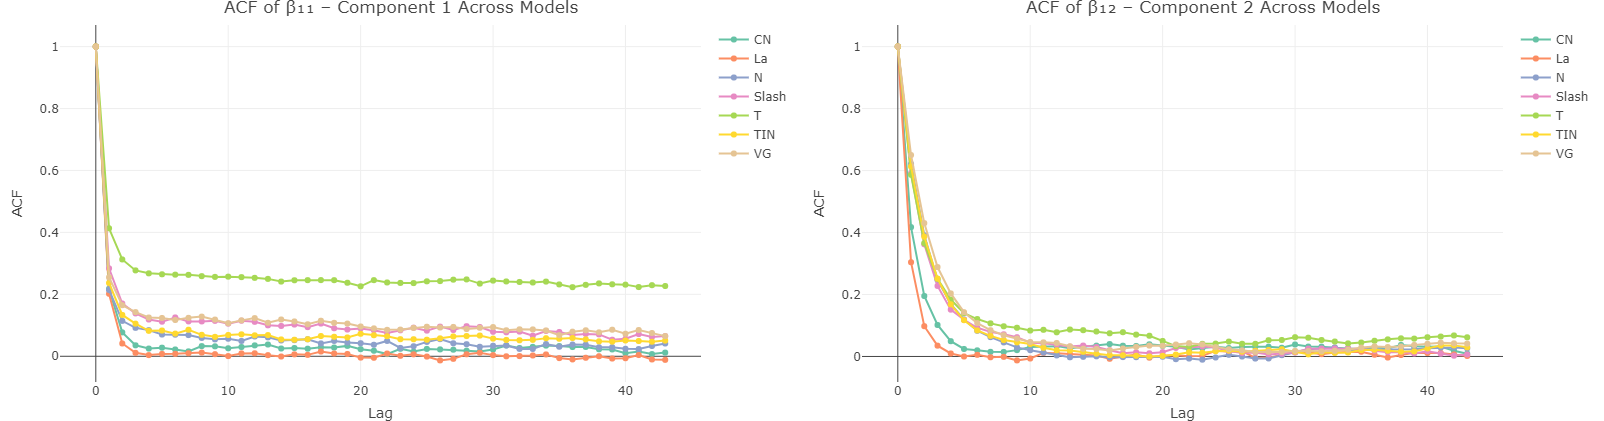
\includegraphics[width=1.1\linewidth]{image (10).png} \\
    \vspace{1em}
    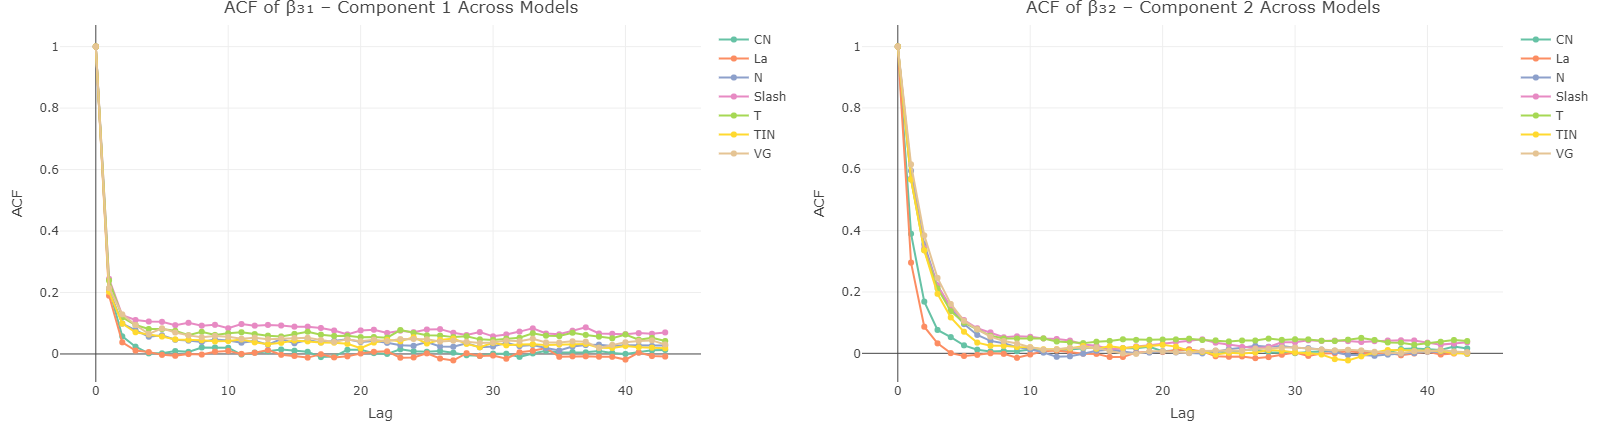
\includegraphics[width=1.1\linewidth]{image (12).png}
    \caption{ACF plots for some of the parameters across models}
    \label{fig:vertical_images}
\end{figure}

\textbf{Interpretation :}
\begin{itemize}
    \item The posterior estimates were examined for four key parameters:
    \begin{itemize}
        \item \( \beta_{11}, \beta_{12} \): Effects of the covariate on the \textbf{mean} in Components 1 and 2.
        \item \( \beta_{31}, \beta_{32} \): Effects of the covariate on the \textbf{autocorrelation structure (ACF)} in Components 1 and 2.
    \end{itemize}
    
    \item Across all error distributions considered (Normal, Student-\( t \), Slash, Contaminated Normal):
    \begin{itemize}
        \item Estimates of \( \beta_{11} \) and \( \beta_{12} \) are \textbf{close to zero}, with \textbf{95\% credible intervals including zero},\\
        \(\Rightarrow\) Indicates \textbf{no significant covariate effect on the mean response}.
        
        \item Estimates of \( \beta_{31} \) and \( \beta_{32} \) have \textbf{posterior means near zero} and \textbf{wide credible intervals},\\
        \(\Rightarrow\) Suggests \textbf{minimal influence of covariates on autocorrelation (spatial/temporal dependence)}.
    \end{itemize}
    
    \item This trend is \textbf{consistent across all mixture model variants}, implying:
    \begin{itemize}
        \item The components mostly capture \textbf{latent structure or background variability}.
        \item Rather than being driven by \textbf{observed covariate effects}.
    \end{itemize}
\end{itemize}

\subsubsection{Posterior Density Plots}

\begin{figure}[H]
    \centering
    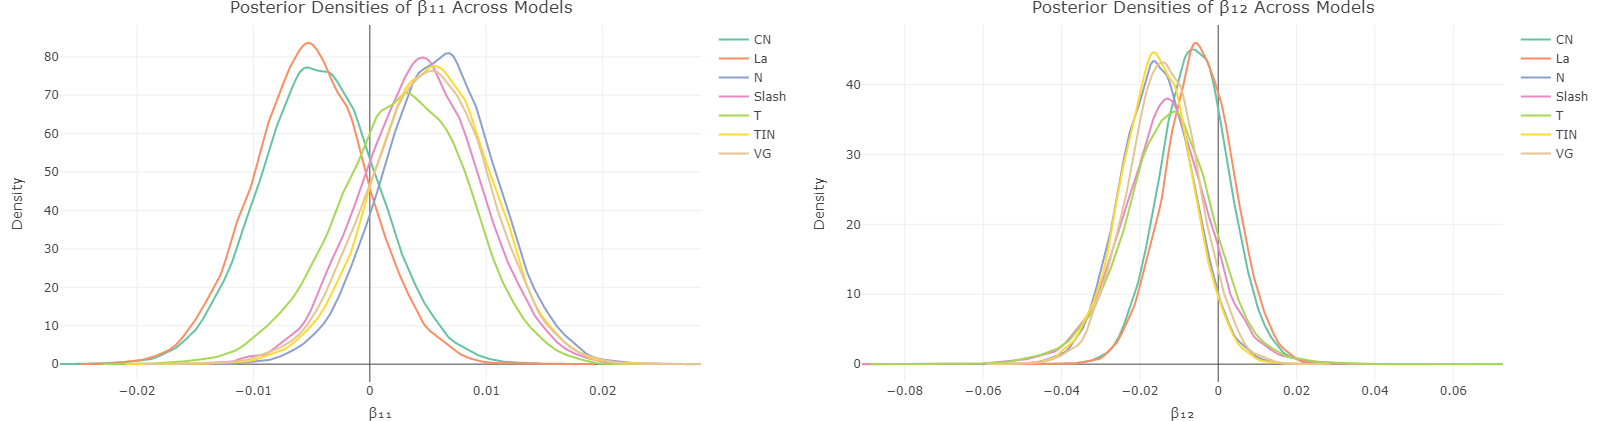
\includegraphics[width=1.2\linewidth]{image (4).png} \\
    \vspace{1.2em}
    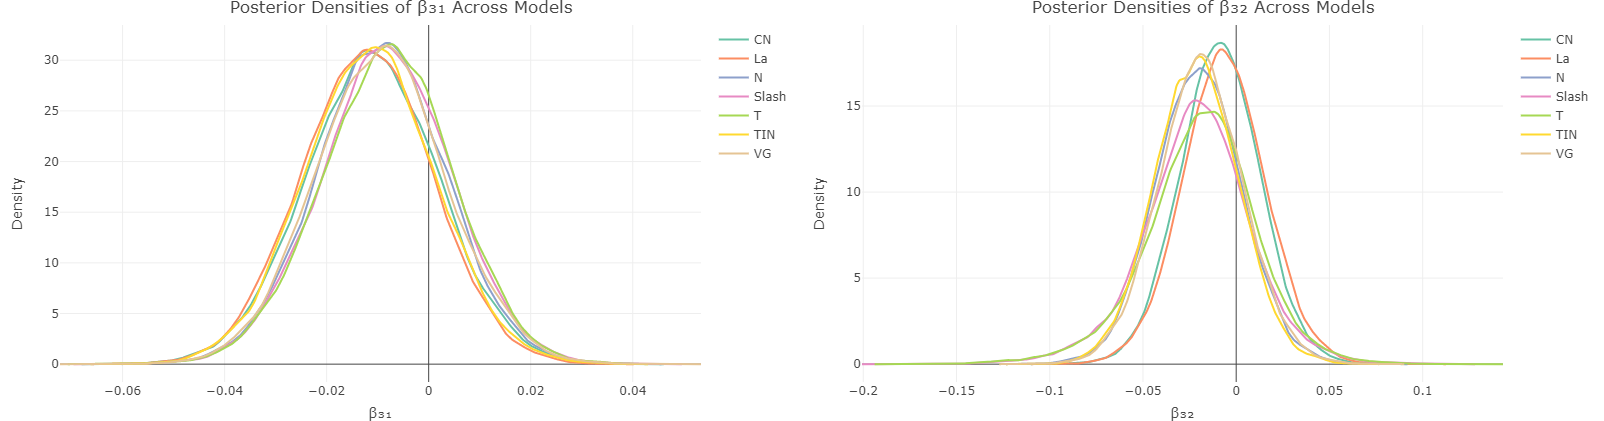
\includegraphics[width=1.2\linewidth]{image (6).png}
    \caption{ACF plots for some of the parameters across models}
    \label{fig:vertical_images}
\end{figure}

\textbf{Interpretation:}
\begin{itemize}
    \item \textbf{Model Robustness:} The posterior densities of $\beta_{11}, \beta_{12}, \beta_{21}, \beta_{22}$ across all models (CN, La, Slash, T, TIN, VG) are largely overlapping, indicating that parameter estimates are robust to the choice of error distribution.
    
    \item \textbf{Centered Around Zero:} Most of the densities are sharply peaked around zero, suggesting that the corresponding covariates have minimal or no significant effect on the response variable in both mixture components.
    
    \item \textbf{Tail Behavior:} Heavier-tailed distributions like Slash, T, and VG show slightly wider posterior spreads, reflecting greater uncertainty, but the central tendency remains consistent across models.
    
    \item \textbf{Inference Consistency:} The high overlap among models implies that the underlying inference drawn from the regression parameters remains consistent, supporting model reliability regardless of error assumptions.
\end{itemize}

\subsubsection{Trace Plots}
\begin{figure}[H]
    \centering
    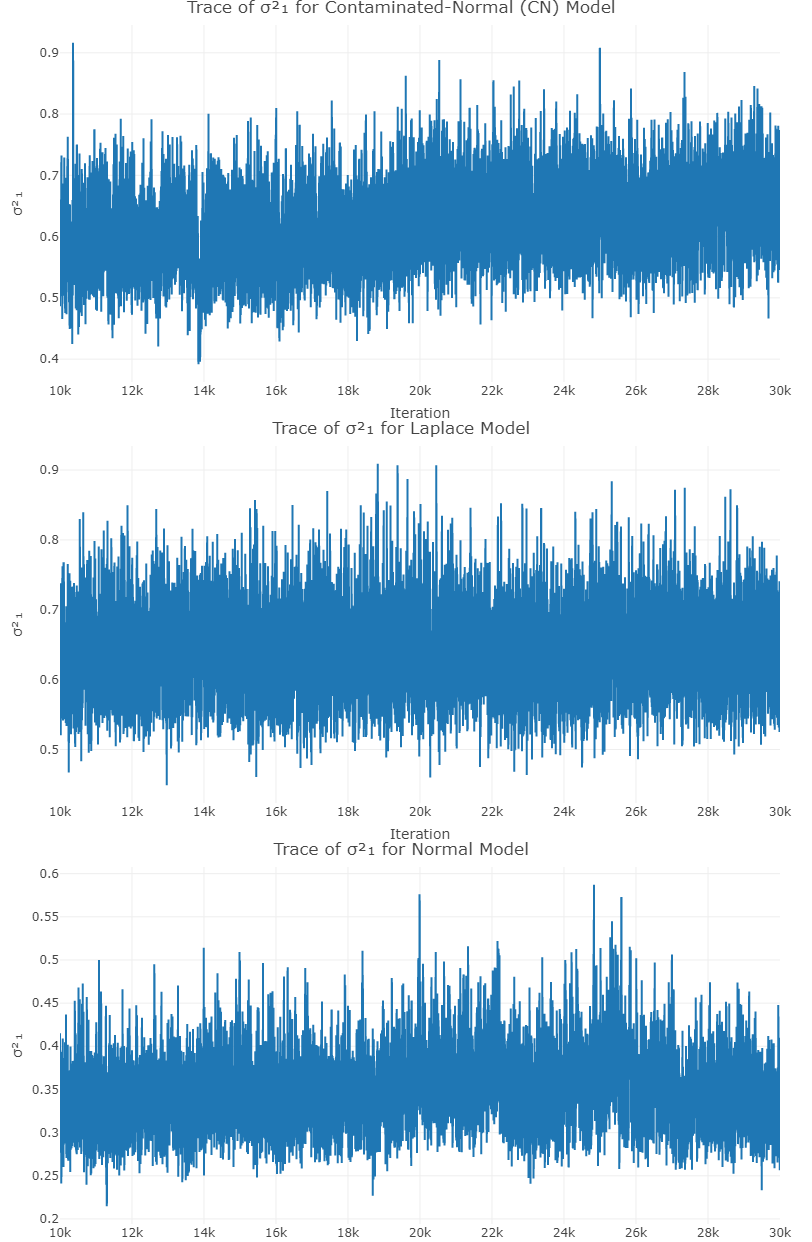
\includegraphics[width=0.6\textwidth]{trace plot.png}
    \caption{Trace plots for CN, Laplace and Normal Models}
    \label{fig:image1}
\end{figure}

\vspace{2em}

\textbf{Interpretation:}\\

\vspace{0.5em}
\noindent
The trace plots of $\sigma^2_1$ under the \textbf{Contaminated Normal}, \textbf{Laplace}, and \textbf{Normal} models exhibit desirable MCMC behavior. All three show good mixing and stationarity, with the Markov chains fluctuating around a stable mean without evident trends or drifts. The Normal model trace is particularly tight and centered, indicating strong convergence with low autocorrelation. The Laplace and Contaminated Normal models also display consistent sampling, suggesting that the posterior distributions for $\sigma^2_1$ have been adequately explored under these models. These results indicate reliable and stable parameter estimation for these three error distributions.

\newpage

\section{Conclusion}

This paper introduces a fully Bayesian approach to the Mixture of Experts (MoE) model using the Scale Mixture of Normal (SMN) distributions, with the capability to handle left and right censoring of the response variable. By leveraging conjugate and weakly informative priors, we have derived explicit full conditional posterior distributions for parameter estimation. The use of the Ultimate Pólya-Gamma (UPG) data-augmentation method has proven efficient in Bayesian estimation of gating parameters. Furthermore, we have proposed an effective scheme for sampling the indexing parameter under various scenarios. 

\vspace{1em}

\noindent
Our simulation results demonstrate that the Bayesian approach outperforms traditional likelihood-based inference, particularly in cases with censored data. Additionally, analysis of real data suggests that the proposed model exhibits robustness against outliers, making it a promising tool for applications involving censored and heavy-tailed data.
\section{Acknowledgment}
We would like to express our sincere gratitude to our supervisor, Dr. Arnab Hazra, for his invaluable guidance and support throughout this project. His expertise and constant encouragement played a key role in the success of this work. We are deeply appreciative of his contributions. We gratefully acknowledge the contributions of Elham Mirfarah, Mehrdad Naderi, Tsung-I Lin, and Wan-Lun Wang, whose work in the referenced paper served as a foundation and inspiration for this project.

\section{Our Contribution}
\begin{itemize}
    \item \textbf{Finding papers:} Ahana Bose, Sneha Karmakar, Sohini Bhadra, Rishikesh Dargad
    \item \textbf{Data Application:} Rishikesh Dargad, Ahana Bose, Sneha Karmakar, Sohini Bhadra
    \item \textbf{Simulation Study:} Sohini Bhadra, Rishikesh Dargad
    \item \textbf{Tables and Plots:} Rishikesh Dargad
    \item \textbf{Report Writing:} Sneha Karmakar, Ahana Bose
\end{itemize}
\end{document}